\documentclass[11pt]{article}
\usepackage[a4paper,margin=20mm,headsep=6mm]{geometry}
\usepackage{amsmath,amssymb}
\usepackage[T1]{fontenc}
\usepackage{lmodern}
\usepackage{xcolor}
\usepackage{tikz}
\usetikzlibrary{arrows.meta}
\usepackage[most]{tcolorbox}
\usepackage{enumitem}
\usepackage{fancyhdr}
\usepackage{needspace}
\usepackage{lastpage}
\definecolor{chalk}{HTML}{2F6F8F}
\definecolor{chalkdk}{HTML}{24576F}
\definecolor{amber}{HTML}{D98A3D}
\definecolor{ink}{HTML}{1A2B34}
\definecolor{inksoft}{HTML}{4A5F68}
\definecolor{paper}{HTML}{F6F4EF}
\definecolor{line}{HTML}{DFE3E0}
\color{ink}
\setlength{\parindent}{0pt}\setlength{\parskip}{3pt}
\pagestyle{fancy}\fancyhf{}
\renewcommand{\headrulewidth}{0.4pt}
\renewcommand{\headrule}{\hbox to\headwidth{\color{line}\leaders\hrule height 0.4pt\hfill}}
\lhead{\small\color{inksoft}\textsc{Quadratics : Chapters 5 \& 7}}
\rhead{\small\color{inksoft}Year 10 Methods : Question Booklet}
\cfoot{\small\color{inksoft}Page \thepage\ of \pageref{LastPage}}
\newcommand{\partband}[2]{\clearpage
  \begin{tcolorbox}[enhanced,colback=chalkdk,colframe=chalkdk,boxrule=0pt,left=14pt,right=14pt,top=12pt,bottom=12pt,arc=4pt]
   {\color{white}\Large\bfseries\textsf{#1}}\\[2pt]{\color{white}\textsf{#2}}\end{tcolorbox}\vspace{4pt}}
\newcommand{\sectionband}[3]{\needspace{5\baselineskip}\vspace{6pt}
  \begin{tcolorbox}[enhanced,colback=chalk,colframe=chalk,boxrule=0pt,left=12pt,right=12pt,top=8pt,bottom=8pt,arc=4pt,
      overlay={\node[anchor=east,text=white,opacity=0.9] at ([xshift=-12pt]frame.east) {\small\textsf{#3}};}]
    {\color{white}\large\bfseries\textsf{#1}\quad #2}\end{tcolorbox}}
\newtcolorbox{refbox}{enhanced,breakable,colback=paper,colframe=line,boxrule=0.6pt,left=12pt,right=12pt,top=8pt,bottom=8pt,arc=3pt}
\newtcolorbox{workedbox}{enhanced,breakable,colback=chalk!6,colframe=chalk!55,boxrule=0.7pt,left=12pt,right=12pt,top=8pt,bottom=8pt,arc=3pt,borderline west={3pt}{0pt}{chalk}}
\newcommand{\worklines}[1]{\par\vspace{2pt}\foreach \n in {1,...,#1}{\vspace{9pt}\noindent\textcolor{line!140!white}{\rule{\linewidth}{0.3pt}}\par}\vspace{2pt}}
\tikzset{fig/.style={line join=round,>=Stealth}}
% ---------- Figure macros (schematic, not to scale) ----------
\newcommand{\figAxes}{\draw[chalkdk!45,->](-2.6,0)--(2.9,0)node[right,font=\scriptsize,ink]{$x$};
  \draw[chalkdk!45,->](0,-2.2)--(0,2.5)node[above,font=\scriptsize,ink]{$y$};}
% area model for expanding: (#1 #2)(#3 #4)
\newcommand{\figAreaModel}[4]{\begin{center}\begin{tikzpicture}[fig,scale=0.85,font=\small]
  \draw[chalkdk,thick](0,0)rectangle(3.4,2.2);\draw[chalkdk](2.1,0)--(2.1,2.2);\draw[chalkdk](0,1.3)--(3.4,1.3);
  \node[above,font=\small]at(1.05,2.25){#1};\node[above,font=\small]at(2.75,2.25){#2};
  \node[left,font=\small]at(-0.05,1.75){#3};\node[left,font=\small]at(-0.05,0.65){#4};
\end{tikzpicture}\end{center}}
% single-bracket area model: #1 x (#2 + #3)
\newcommand{\figAreaOne}[3]{\begin{center}\begin{tikzpicture}[fig,scale=0.85,font=\small]
  \draw[chalkdk,thick](0,0)rectangle(3.4,1.15);\draw[chalkdk](2.1,0)--(2.1,1.15);
  \node[above,font=\small]at(1.05,1.2){#2};\node[above,font=\small]at(2.75,1.2){#3};
  \node[left,font=\small]at(-0.05,0.575){#1};
\end{tikzpicture}\end{center}}
% difference of two squares visual
\newcommand{\figDOPS}{\begin{center}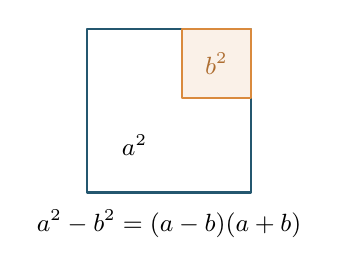
\begin{tikzpicture}[fig,scale=0.8,font=\small]
  \draw[chalkdk,thick](0,0)rectangle(2.6,2.6);\draw[amber,thick,fill=amber!12](1.5,1.5)rectangle(2.6,2.6);
  \node at(0.75,0.75){$a^2$};\node[amber!80!black]at(2.05,2.05){$b^2$};
  \node[below]at(1.3,-0.12){$a^2-b^2=(a-b)(a+b)$};
\end{tikzpicture}\end{center}}
% completing the square visual
\newcommand{\figCompSq}{\begin{center}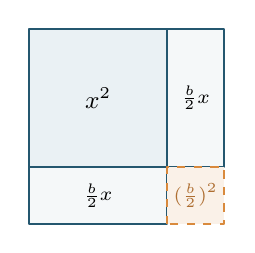
\begin{tikzpicture}[fig,scale=0.8,font=\small]
  \draw[chalkdk,thick,fill=chalk!10](0,0)rectangle(2.2,2.2);\node at(1.1,1.1){$x^2$};
  \draw[chalkdk,thick,fill=chalk!5](2.2,0)rectangle(3.1,2.2);\node[font=\scriptsize]at(2.65,1.1){$\frac{b}{2}x$};
  \draw[chalkdk,thick,fill=chalk!5](0,-0.9)rectangle(2.2,0);\node[font=\scriptsize]at(1.1,-0.45){$\frac{b}{2}x$};
  \draw[amber,thick,dashed,fill=amber!12](2.2,-0.9)rectangle(3.1,0);\node[font=\scriptsize,amber!80!black]at(2.65,-0.45){$(\frac{b}{2})^2$};
\end{tikzpicture}\end{center}}
% rectangle with dimensions and area
\newcommand{\figRect}[3]{\begin{center}\begin{tikzpicture}[fig,scale=0.8,font=\small]
  \draw[chalkdk,very thick](0,0)rectangle(3.6,2.0);
  \node[below]at(1.8,-0.1){#2};\node[left]at(-0.08,1.0){#1};\node[chalk]at(1.8,1.0){#3};
\end{tikzpicture}\end{center}}
% parabola with two roots labelled
\newcommand{\figParabRoots}[2]{\begin{center}\begin{tikzpicture}[fig,scale=0.85]
  \figAxes \draw[chalkdk,very thick,domain=-1.9:1.9,samples=60,smooth]plot(\x,{\x*\x-1.6});
  \fill[amber](-1.265,0)circle(1.6pt);\fill[amber](1.265,0)circle(1.6pt);
  \node[font=\scriptsize,below left]at(-1.265,0){#1};\node[font=\scriptsize,below right]at(1.265,0){#2};
\end{tikzpicture}\end{center}}
% parabola touching axis (one root)
\newcommand{\figParabTouch}[1]{\begin{center}\begin{tikzpicture}[fig,scale=0.85]
  \figAxes \draw[chalkdk,very thick,domain=-1.6:1.6,samples=60,smooth]plot(\x,{\x*\x});
  \fill[amber](0,0)circle(1.7pt);\node[font=\scriptsize,below right]at(0.1,-0.05){#1};
\end{tikzpicture}\end{center}}
% parabola with no real roots
\newcommand{\figNoRoots}{\begin{center}\begin{tikzpicture}[fig,scale=0.85]
  \figAxes \draw[chalkdk,very thick,domain=-1.7:1.7,samples=60,smooth]plot(\x,{\x*\x+0.8});
  \node[font=\scriptsize,chalk,right]at(1.0,2.0){no $x$-intercepts};
\end{tikzpicture}\end{center}}
% parabola with turning point labelled
\newcommand{\figParabTP}[1]{\begin{center}\begin{tikzpicture}[fig,scale=0.85]
  \figAxes \draw[chalkdk,very thick,domain=-1.5:1.9,samples=60,smooth]plot({\x+0.4},{(\x)*(\x)-1.0});
  \fill[amber](0.4,-1.0)circle(1.7pt);\node[font=\scriptsize,below right,amber!80!black]at(0.5,-1.05){#1};
  \draw[chalkdk!50,dashed](0.4,-1.0)--(0.4,2.2);
\end{tikzpicture}\end{center}}
% fully labelled parabola for reading features
\newcommand{\figParabLabelled}{\begin{center}\begin{tikzpicture}[fig,scale=0.95]
  \figAxes \draw[chalkdk,very thick,domain=-1.6:1.6,samples=60,smooth]plot(\x,{\x*\x-1.2});
  \fill[amber](0,-1.2)circle(1.7pt);\node[font=\scriptsize,below right]at(0.08,-1.25){TP};
  \draw[chalkdk!50,dashed](0,-1.2)--(0,2.2);\node[font=\scriptsize,chalk,right]at(0.06,2.0){axis};
  \fill[chalk](0,-1.2)circle(0pt);
  \fill[amber](-1.095,0)circle(1.5pt);\fill[amber](1.095,0)circle(1.5pt);
\end{tikzpicture}\end{center}}
% upright vs inverted
\newcommand{\figUpDown}{\begin{center}\begin{tikzpicture}[fig,scale=0.8]
  \begin{scope}\figAxes\draw[chalkdk,very thick,domain=-1.4:1.4,samples=50,smooth]plot(\x,{1.1*\x*\x-0.8});
   \node[font=\scriptsize,chalk]at(0,-1.9){upright};\end{scope}
  \begin{scope}[xshift=6.2cm]\figAxes\draw[amber,very thick,domain=-1.4:1.4,samples=50,smooth]plot(\x,{-\x*\x+1.0});
   \node[font=\scriptsize,amber!80!black]at(0,-1.9){inverted};\end{scope}
\end{tikzpicture}\end{center}}
% wide vs narrow
\newcommand{\figWideNarrow}{\begin{center}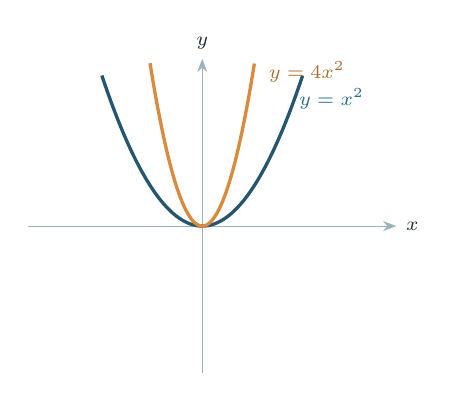
\begin{tikzpicture}[fig,scale=0.85]
  \figAxes \draw[chalkdk,very thick,domain=-1.5:1.5,samples=60,smooth]plot(\x,{\x*\x});
  \draw[amber,very thick,domain=-0.78:0.78,samples=60,smooth]plot(\x,{4*\x*\x});
  \node[font=\scriptsize,chalk,right]at(1.3,1.9){$y=x^2$};\node[font=\scriptsize,amber!80!black,right]at(0.85,2.3){$y=4x^2$};
\end{tikzpicture}\end{center}}
% discriminant three cases
\newcommand{\figDiscThree}{\begin{center}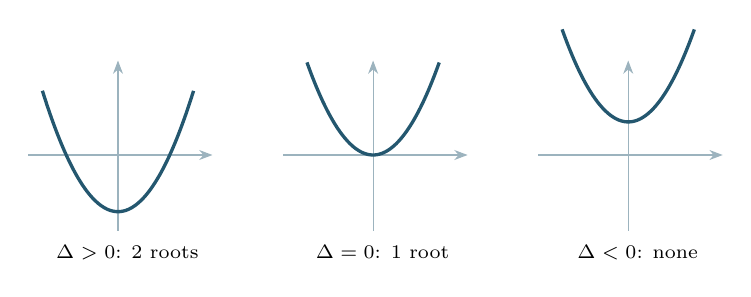
\begin{tikzpicture}[fig,scale=0.6,font=\scriptsize]
 \foreach \s/\lab/\off in {1/{$\Delta>0$: 2 roots}/0, 2/{$\Delta=0$: 1 root}/5.4, 3/{$\Delta<0$: none}/10.8}{
  \begin{scope}[xshift=\off cm]
   \draw[chalkdk!45,->](-1.9,0)--(2.0,0);\draw[chalkdk!45,->](0,-1.6)--(0,2.0);
   \ifnum\s=1 \draw[chalkdk,very thick,domain=-1.6:1.6,samples=50,smooth]plot(\x,{\x*\x-1.2});\fi
   \ifnum\s=2 \draw[chalkdk,very thick,domain=-1.4:1.4,samples=50,smooth]plot(\x,{\x*\x});\fi
   \ifnum\s=3 \draw[chalkdk,very thick,domain=-1.4:1.4,samples=50,smooth]plot(\x,{\x*\x+0.7});\fi
   \node[below]at(0.2,-1.7){\lab};
  \end{scope}}
\end{tikzpicture}\end{center}}
% line and parabola intersecting
\newcommand{\figLinePara}{\begin{center}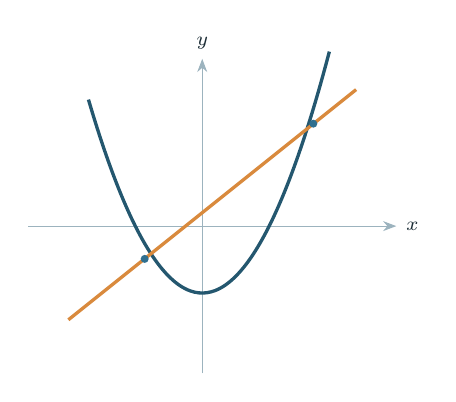
\begin{tikzpicture}[fig,scale=0.85]
  \figAxes \draw[chalkdk,very thick,domain=-1.7:1.9,samples=60,smooth]plot(\x,{\x*\x-1.0});
  \draw[amber,very thick,domain=-2.0:2.3]plot(\x,{0.8*\x+0.2});
  \fill[chalk](-0.86,-0.49)circle(1.7pt);\fill[chalk](1.66,1.53)circle(1.7pt);
\end{tikzpicture}\end{center}}
\newcommand{\figLineHoriz}{\begin{center}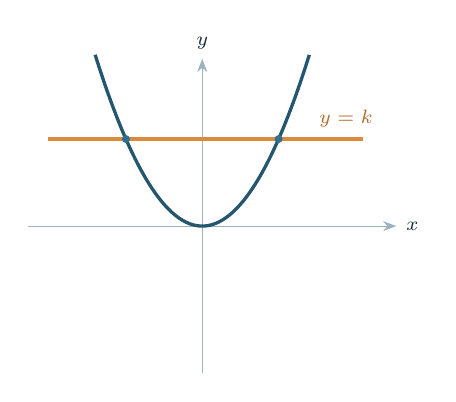
\begin{tikzpicture}[fig,scale=0.85]
  \figAxes \draw[chalkdk,very thick,domain=-1.6:1.6,samples=60,smooth]plot(\x,{\x*\x});
  \draw[amber,very thick](-2.3,1.3)--(2.4,1.3);\node[font=\scriptsize,amber!80!black,right]at(1.6,1.6){$y=k$};
  \fill[chalk](-1.14,1.3)circle(1.7pt);\fill[chalk](1.14,1.3)circle(1.7pt);
\end{tikzpicture}\end{center}}
\newcommand{\figNoIntersect}{\begin{center}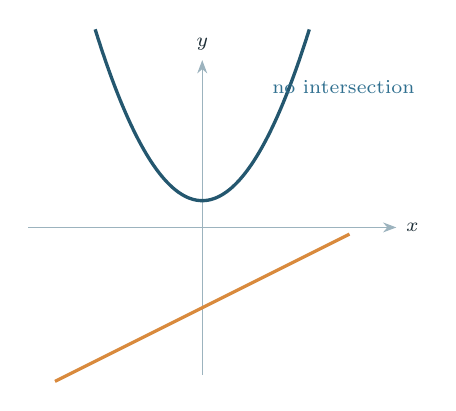
\begin{tikzpicture}[fig,scale=0.85]
  \figAxes \draw[chalkdk,very thick,domain=-1.6:1.6,samples=60,smooth]plot(\x,{\x*\x+0.4});
  \draw[amber,very thick,domain=-2.2:2.2]plot(\x,{0.5*\x-1.2});
  \node[font=\scriptsize,chalk,right]at(0.9,2.1){no intersection};
\end{tikzpicture}\end{center}}
\newcommand{\figTangent}{\begin{center}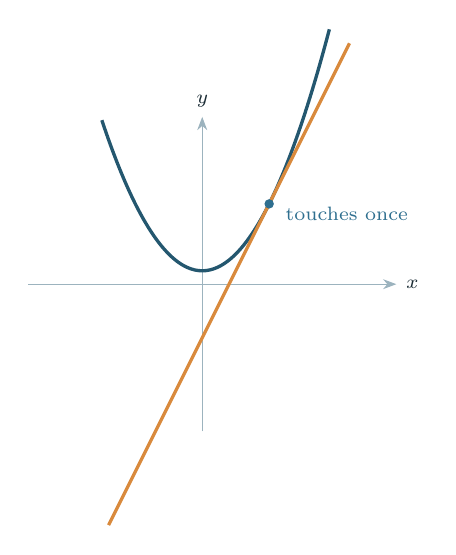
\begin{tikzpicture}[fig,scale=0.85]
  \figAxes \draw[chalkdk,very thick,domain=-1.5:1.9,samples=60,smooth]plot(\x,{\x*\x+0.2});
  \draw[amber,very thick,domain=-1.4:2.2]plot(\x,{2*\x-0.8});
  \fill[chalk](1,1.2)circle(2pt);\node[font=\scriptsize,chalk,right]at(1.1,1.05){touches once};
\end{tikzpicture}\end{center}}
% projectile height-time
\newcommand{\figProjectile}{\begin{center}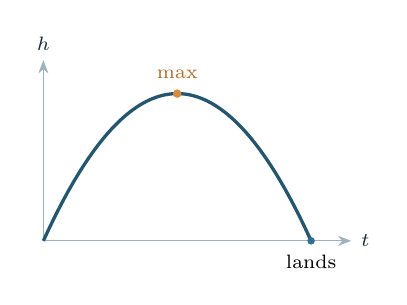
\begin{tikzpicture}[fig,scale=0.85]
  \draw[chalkdk!45,->](0,0)--(4.6,0)node[right,font=\scriptsize,ink]{$t$};
  \draw[chalkdk!45,->](0,0)--(0,2.7)node[above,font=\scriptsize,ink]{$h$};
  \draw[chalkdk,very thick,domain=0:4,samples=60,smooth]plot(\x,{0.55*\x*(4-\x)});
  \fill[amber](2,2.2)circle(1.8pt);\node[font=\scriptsize,above,amber!80!black]at(2,2.28){max};
  \fill[chalk](4,0)circle(1.6pt);\node[font=\scriptsize,below]at(4,-0.06){lands};
\end{tikzpicture}\end{center}}
\newcommand{\figArch}{\begin{center}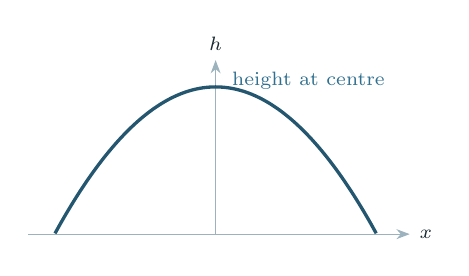
\begin{tikzpicture}[fig,scale=0.85]
  \draw[chalkdk!45,->](-2.8,0)--(2.9,0)node[right,font=\scriptsize,ink]{$x$};
  \draw[chalkdk!45,->](0,0)--(0,2.6)node[above,font=\scriptsize,ink]{$h$};
  \draw[chalkdk,very thick,domain=-2.4:2.4,samples=60,smooth]plot(\x,{2.2-0.38*\x*\x});
  \node[font=\scriptsize,chalk,right]at(0.1,2.3){height at centre};
\end{tikzpicture}\end{center}}
% distance-time graph
\newcommand{\figDistTime}{\begin{center}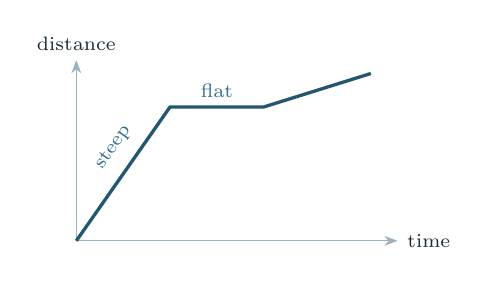
\begin{tikzpicture}[fig,scale=0.85]
  \draw[chalkdk!45,->](0,0)--(4.8,0)node[right,font=\scriptsize,ink]{time};
  \draw[chalkdk!45,->](0,0)--(0,2.7)node[above,font=\scriptsize,ink]{distance};
  \draw[chalkdk,very thick](0,0)--(1.4,2.0)--(2.8,2.0)--(4.4,2.5);
  \node[font=\scriptsize,chalk,rotate=55]at(0.55,1.4){steep};
  \node[font=\scriptsize,chalk,above]at(2.1,2.0){flat};
\end{tikzpicture}\end{center}}
% chord vs tangent
\newcommand{\figChordTangent}{\begin{center}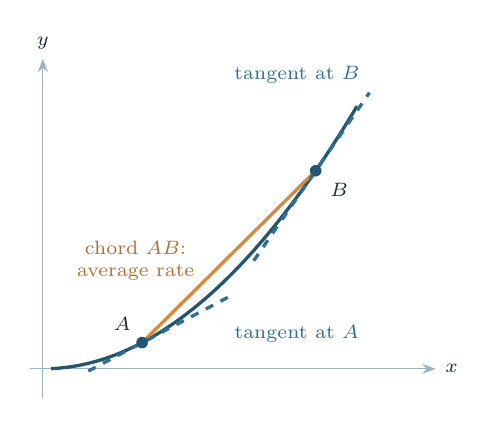
\begin{tikzpicture}[fig,scale=1.05]
  \draw[chalkdk!45,->](-0.15,0)--(4.75,0)node[right,font=\scriptsize,ink]{$x$};
  \draw[chalkdk!45,->](0,-0.35)--(0,3.75)node[above,font=\scriptsize,ink]{$y$};
  \draw[chalkdk,very thick,domain=0.1:3.8,samples=70,smooth]plot(\x,{0.22*\x*\x});
  % chord AB -- the average rate of change between A and B
  \draw[amber,very thick](1.2,0.3168)--(3.3,2.3958);
  \node[font=\scriptsize,amber!80!black,above left,align=center]at(1.95,0.95){chord $AB$:\\average rate};
  % tangent at A -- instantaneous rate of change at A
  \draw[chalk,very thick,dashed](0.55,-0.027)--(2.30,0.897);
  \node[font=\scriptsize,chalk,right]at(2.20,0.42){tangent at $A$};
  % tangent at B -- instantaneous rate of change at B
  \draw[chalk,very thick,dashed](2.55,1.307)--(3.95,3.340);
  \node[font=\scriptsize,chalk,above left]at(3.95,3.34){tangent at $B$};
  % the two points
  \fill[chalkdk](1.2,0.3168)circle(2pt);\node[font=\scriptsize,ink,above left]at(1.18,0.34){$A$};
  \fill[chalkdk](3.3,2.3958)circle(2pt);\node[font=\scriptsize,ink,below right]at(3.36,2.36){$B$};
\end{tikzpicture}\end{center}}
% direct vs inverse variation
\newcommand{\figVariation}{\begin{center}\begin{tikzpicture}[fig,scale=0.75,font=\scriptsize]
  \begin{scope}\draw[chalkdk!45,->](0,0)--(3.2,0)node[right,ink]{$x$};\draw[chalkdk!45,->](0,0)--(0,2.6)node[above,ink]{$y$};
   \draw[chalkdk,very thick](0,0)--(2.7,2.3);\node[below]at(1.5,-0.25){A};\end{scope}
  \begin{scope}[xshift=5.4cm]\draw[chalkdk!45,->](0,0)--(3.2,0)node[right,ink]{$x$};\draw[chalkdk!45,->](0,0)--(0,2.6)node[above,ink]{$y$};
   \draw[chalkdk,very thick,domain=0.42:2.9,samples=50,smooth]plot(\x,{1.0/\x});\node[below]at(1.5,-0.25){B};\end{scope}
\end{tikzpicture}\end{center}}
% blank sketching grid
\newcommand{\figGridBlank}{\par\vspace{3pt}\begin{center}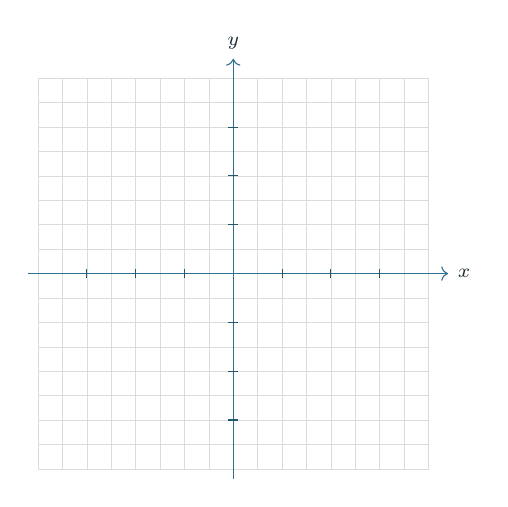
\begin{tikzpicture}[scale=0.62]
  \draw[step=0.5cm,line!120!white,very thin](-4,-4)grid(4,4);
  \draw[chalk,->](-4.2,0)--(4.4,0)node[right,font=\scriptsize,ink]{$x$};
  \draw[chalk,->](0,-4.2)--(0,4.4)node[above,font=\scriptsize,ink]{$y$};
  \foreach \x in {-3,-2,-1,1,2,3}{\draw[chalkdk](\x,-0.1)--(\x,0.1);\draw[chalkdk](-0.1,\x)--(0.1,\x);}
\end{tikzpicture}\end{center}}
\begin{document}
\thispagestyle{empty}
\begin{tikzpicture}[remember picture,overlay]
  \fill[chalk](current page.north west)rectangle([yshift=-64mm]current page.north east);
  \node[anchor=north west,text=white,align=left]at([xshift=20mm,yshift=-19mm]current page.north west)
    {{\Huge\bfseries\textsf{Quadratics}}\\[3mm]{\LARGE\textsf{Student Question Booklet}}\\[3mm]
     {\large\textsf{Chapters 5 \& 7 : Year 10 Mathematical Methods : 2026}}};
\end{tikzpicture}
\vspace{60mm}
\vspace{5mm}
\begin{refbox}
{\bfseries\color{chalkdk}How to use this booklet}\\[2pt]
This booklet covers the whole quadratic story in two parts:
\begin{itemize}[leftmargin=16pt,itemsep=2pt,topsep=3pt]
  \item \textbf{Part A --- Quadratic Algebra (Chapter 5).} Expanding, factorising, and solving quadratic equations.
  \item \textbf{Part B --- Quadratic Functions (Chapter 7).} Parabolas, sketching, applications, rates of change and variation.
\end{itemize}
\vspace{3pt}For every section you will find:
\begin{itemize}[leftmargin=16pt,itemsep=2pt,topsep=3pt]
  \item \textbf{Worked examples} --- fully solved, with a diagram where it helps, plus the matching textbook example numbers and pages.
  \item \textbf{Question sets} --- what to practise, grouped by \textit{Building Understanding}, \textit{Fluency}, \textit{Problem-solving}, \textit{Reasoning} and \textit{Enrichment}, with page numbers. Find them in your own textbook.
  \item \textbf{Hurdle questions} --- five questions you \textbf{must} be able to do to pass the section, with working space.
\end{itemize}
\vspace{2pt}{\small\color{inksoft}Diagrams are schematic (not to scale). Sections marked \textsf{10A} are extension. Always show full working --- in algebra the method earns the marks.}
\end{refbox}
\vspace{3mm}{\small\color{inksoft}Page references are to \emph{Essential Mathematics for the Victorian Curriculum 10 \& 10A}, 3rd ed. Question sets belong to the textbook; the worked examples, diagrams and hurdle questions are original material written for this course.}


\partband{Part A --- Quadratic Algebra}{Chapter 5 : expanding, factorising and solving quadratic equations}

\sectionband{5A}{Expanding expressions}{CONSOLIDATING}

\begin{refbox}
{\bfseries\color{chalkdk}Textbook worked examples}\;\textcolor{inksoft}{\small(cross-reference in your textbook)}\\[3pt]
\begin{itemize}[leftmargin=16pt,itemsep=1pt,topsep=2pt]
  \item \textbf{Example 1} --- Expanding simple expressions \textcolor{inksoft}{(p.\,417)}
  \item \textbf{Example 2} --- Expanding binomial products, perfect squares and DOPS \textcolor{inksoft}{(p.\,418)}
  \item \textbf{Example 3} --- Expanding more binomial products \textcolor{inksoft}{(p.\,418)}
\end{itemize}
\vspace{4pt}{\bfseries\color{chalkdk}Question sets}\;\textcolor{inksoft}{\small(practise from your textbook)}\\[3pt]
\begin{itemize}[leftmargin=16pt,itemsep=1pt,topsep=2pt]
  \item \textbf{Building Understanding:} Q1--3 \textcolor{inksoft}{(p.\,417)}
  \item \textbf{Fluency:} Q1--5 \textcolor{inksoft}{(p.\,419--420)}
  \item \textbf{Problem-solving:} Q6--9 \textcolor{inksoft}{(p.\,420)}
  \item \textbf{Reasoning:} Q10--13 \textcolor{inksoft}{(p.\,421)}
  \item \textbf{Enrichment: Expanding to prove:} Q14 \textcolor{inksoft}{(p.\,421)}
\end{itemize}\end{refbox}

\vspace{4pt}{\bfseries\color{chalkdk}\large Worked examples}\;\textcolor{inksoft}{\small(study the method, then try the hurdles)}\par

\needspace{7\baselineskip}\begin{workedbox}

{\bfseries\color{chalkdk}Expanding a binomial product}\par\vspace{3pt}

Expand and simplify $(x+5)(x-2)$.\par\vspace{2pt}

\figAreaModel{$x$}{$+5$}{$x$}{$-2$}

{\bfseries Solution.}\ Multiply every term in the first bracket by every term in the second (FOIL), then collect like terms. \begin{align*}(x+5)(x-2)&=x^2-2x+5x-10\\&=x^2+3x-10.\end{align*}

\end{workedbox}

\needspace{7\baselineskip}\begin{workedbox}

{\bfseries\color{chalkdk}Perfect square and difference of squares}\par\vspace{3pt}

Expand \textbf{(a)} $(x+4)^2$ and \textbf{(b)} $(x-3)(x+3)$.\par\vspace{2pt}

{\bfseries Solution.}\ \textbf{(a)} $(a+b)^2=a^2+2ab+b^2$: \[(x+4)^2=x^2+8x+16.\] \textbf{(b)} $(a-b)(a+b)=a^2-b^2$, so the middle terms cancel: \[(x-3)(x+3)=x^2-9.\]

\end{workedbox}

\vspace{6pt}{\bfseries\color{amber}\large Hurdle questions --- Section 5A}\;\textcolor{inksoft}{\small(show all working)}\par\vspace{2pt}

\begin{enumerate}[leftmargin=20pt,itemsep=5pt,topsep=3pt,label=\textbf{H\arabic*.}]

\needspace{7\baselineskip}

  \item Expand and simplify:

  \begin{enumerate}[leftmargin=20pt,itemsep=3pt,topsep=3pt,label=\textbf{(\alph*)}]

    \item $3(2x-5)$

    \figAreaOne{$3$}{$2x$}{$-5$}

    \worklines{2}

    \item $-2x(4x+7)$

    \figAreaOne{$-2x$}{$4x$}{$+7$}

    \worklines{2}

  \end{enumerate}

\needspace{7\baselineskip}

  \item Expand and simplify $(x+4)(x-3)$.

  \figAreaModel{$x$}{$+4$}{$x$}{$-3$}

  \worklines{3}

\needspace{7\baselineskip}

  \item Expand the perfect square $(2x+5)^2$.

  \figAreaModel{$2x$}{$+5$}{$2x$}{$+5$}

  \worklines{3}

\needspace{7\baselineskip}

  \item Expand the difference of perfect squares $(3x-2)(3x+2)$.

  \figDOPS

  \worklines{3}

\needspace{7\baselineskip}

  \item Expand and simplify $(x+3)(x-2)-(x-1)(x+4)$.

  \worklines{4}

\end{enumerate}\clearpage

\sectionband{5B}{Factorising expressions}{CORE}

\begin{refbox}
{\bfseries\color{chalkdk}Textbook worked examples}\;\textcolor{inksoft}{\small(cross-reference in your textbook)}\\[3pt]
\begin{itemize}[leftmargin=16pt,itemsep=1pt,topsep=2pt]
  \item \textbf{Example 4} --- Taking out common factors \textcolor{inksoft}{(p.\,423)}
  \item \textbf{Example 5} --- Factorising a difference of two squares \textcolor{inksoft}{(p.\,424)}
  \item \textbf{Example 6} --- Factorising a DOPS using surds \textcolor{inksoft}{(p.\,424)}
  \item \textbf{Example 7} --- Factorising by grouping \textcolor{inksoft}{(p.\,425)}
\end{itemize}
\vspace{4pt}{\bfseries\color{chalkdk}Question sets}\;\textcolor{inksoft}{\small(practise from your textbook)}\\[3pt]
\begin{itemize}[leftmargin=16pt,itemsep=1pt,topsep=2pt]
  \item \textbf{Building Understanding:} Q1--3 \textcolor{inksoft}{(p.\,423)}
  \item \textbf{Fluency:} Q1--6 \textcolor{inksoft}{(p.\,425--426)}
  \item \textbf{Problem-solving:} Q7--10 \textcolor{inksoft}{(p.\,426)}
  \item \textbf{Reasoning:} Q11--14 \textcolor{inksoft}{(p.\,427)}
  \item \textbf{Enrichment: Hidden difference of two squares:} Q15--16 \textcolor{inksoft}{(p.\,427)}
\end{itemize}\end{refbox}

\vspace{4pt}{\bfseries\color{chalkdk}\large Worked examples}\;\textcolor{inksoft}{\small(study the method, then try the hurdles)}\par

\needspace{7\baselineskip}\begin{workedbox}

{\bfseries\color{chalkdk}Taking out a common factor}\par\vspace{3pt}

Factorise $12x^2-18x$.\par\vspace{2pt}

{\bfseries Solution.}\ The highest common factor of $12x^2$ and $18x$ is $6x$. Divide each term by it: \[12x^2-18x=6x(2x-3).\]

\end{workedbox}

\needspace{7\baselineskip}\begin{workedbox}

{\bfseries\color{chalkdk}Difference of two squares}\par\vspace{3pt}

Factorise $4x^2-25$.\par\vspace{2pt}

\figDOPS

{\bfseries Solution.}\ Write each term as a square: $4x^2=(2x)^2$ and $25=5^2$. Then use $a^2-b^2=(a-b)(a+b)$: \[4x^2-25=(2x-5)(2x+5).\]

\end{workedbox}
\newpage
\vspace{6pt}{\bfseries\color{amber}\large Hurdle questions --- Section 5B}\;\textcolor{inksoft}{\small(show all working)}\par\vspace{2pt}

\begin{enumerate}[leftmargin=20pt,itemsep=5pt,topsep=3pt,label=\textbf{H\arabic*.}]

\needspace{7\baselineskip}

  \item Factorise by taking out the highest common factor:

  \begin{enumerate}[leftmargin=20pt,itemsep=3pt,topsep=3pt,label=\textbf{(\alph*)}]

    \item $6x+18$

    \figAreaOne{$6$}{$x$}{$+3$}

    \worklines{2}

    \item $8x^2-12x$

    \figAreaOne{$4x$}{$2x$}{$-3$}

    \worklines{2}

  \end{enumerate}

\needspace{7\baselineskip}

  \item Factorise the difference of two squares $x^2-49$.

  \figDOPS

  \worklines{3}

\needspace{7\baselineskip}

  \item Factorise $9x^2-25$.

  \figDOPS

  \worklines{3}

\needspace{7\baselineskip}

  \item Factorise $x^2-7$ using surds.

  \worklines{4}

\needspace{7\baselineskip}

  \item Factorise by grouping: $x^2+3x+2x+6$.

  \worklines{4}

\end{enumerate}\clearpage

\sectionband{5C}{Multiplying and dividing algebraic fractions}{CORE}

\begin{refbox}
{\bfseries\color{chalkdk}Textbook worked examples}\;\textcolor{inksoft}{\small(cross-reference in your textbook)}\\[3pt]
\begin{itemize}[leftmargin=16pt,itemsep=1pt,topsep=2pt]
  \item \textbf{Example 8} --- Cancelling common factors \textcolor{inksoft}{(p.\,429)}
  \item \textbf{Example 9} --- Multiplying and dividing algebraic fractions \textcolor{inksoft}{(p.\,430)}
\end{itemize}
\vspace{4pt}{\bfseries\color{chalkdk}Question sets}\;\textcolor{inksoft}{\small(practise from your textbook)}\\[3pt]
\begin{itemize}[leftmargin=16pt,itemsep=1pt,topsep=2pt]
  \item \textbf{Building Understanding:} Q1--3 \textcolor{inksoft}{(p.\,429)}
  \item \textbf{Fluency:} Q1--4 \textcolor{inksoft}{(p.\,430--431)}
  \item \textbf{Problem-solving:} Q5--8 \textcolor{inksoft}{(p.\,431)}
  \item \textbf{Reasoning:} Q9--11 \textcolor{inksoft}{(p.\,432)}
  \item \textbf{Enrichment: Same or different?:} Q12 \textcolor{inksoft}{(p.\,432)}
\end{itemize}\end{refbox}

\vspace{4pt}{\bfseries\color{chalkdk}\large Worked examples}\;\textcolor{inksoft}{\small(study the method, then try the hurdles)}\par

\needspace{7\baselineskip}\begin{workedbox}

{\bfseries\color{chalkdk}Simplifying by cancelling}\par\vspace{3pt}

Simplify $\dfrac{x^2-4}{x-2}$.\par\vspace{2pt}

{\bfseries Solution.}\ Factorise the numerator as a difference of two squares, then cancel: \[\frac{x^2-4}{x-2}=\frac{(x-2)(x+2)}{x-2}=x+2,\quad x\neq2.\]

\end{workedbox}

\needspace{7\baselineskip}\begin{workedbox}

{\bfseries\color{chalkdk}Multiplying algebraic fractions}\par\vspace{3pt}

Simplify $\dfrac{3x}{4}\times\dfrac{8}{9x^2}$.\par\vspace{2pt}

{\bfseries Solution.}\ Cancel common factors before multiplying: \[\frac{3x}{4}\times\frac{8}{9x^2}=\frac{3x\times 8}{4\times 9x^2}=\frac{24x}{36x^2}=\frac{2}{3x}.\]

\end{workedbox}

\vspace{6pt}{\bfseries\color{amber}\large Hurdle questions --- Section 5C}\;\textcolor{inksoft}{\small(show all working)}\par\vspace{2pt}

\begin{enumerate}[leftmargin=20pt,itemsep=5pt,topsep=3pt,label=\textbf{H\arabic*.}]

\needspace{7\baselineskip}

  \item Simplify by cancelling common factors: $\dfrac{6x^2}{9x}$.

  \worklines{4}

\needspace{7\baselineskip}

  \item Simplify $\dfrac{3(x+2)}{6(x+2)}$.

  \worklines{4}

\needspace{7\baselineskip}

  \item Simplify $\dfrac{x^2-9}{x+3}$.

  \worklines{4}

\needspace{7\baselineskip}

  \item Simplify $\dfrac{2x}{5}\times\dfrac{15}{4x^2}$.

  \worklines{4}

\needspace{7\baselineskip}

  \item Simplify $\dfrac{x+1}{4}\div\dfrac{x+1}{8}$.

  \worklines{4}

\end{enumerate}\clearpage

\sectionband{5D}{Factorising monic quadratic trinomials}{CORE}

\begin{refbox}
{\bfseries\color{chalkdk}Textbook worked examples}\;\textcolor{inksoft}{\small(cross-reference in your textbook)}\\[3pt]
\begin{itemize}[leftmargin=16pt,itemsep=1pt,topsep=2pt]
  \item \textbf{Example 10} --- Factorising trinomials of the form $x^2+bx+c$ \textcolor{inksoft}{(p.\,434)}
  \item \textbf{Example 11} --- Simplifying algebraic fractions \textcolor{inksoft}{(p.\,435)}
\end{itemize}
\vspace{4pt}{\bfseries\color{chalkdk}Question sets}\;\textcolor{inksoft}{\small(practise from your textbook)}\\[3pt]
\begin{itemize}[leftmargin=16pt,itemsep=1pt,topsep=2pt]
  \item \textbf{Building Understanding:} Q1--3 \textcolor{inksoft}{(p.\,434)}
  \item \textbf{Fluency:} Q1--4 \textcolor{inksoft}{(p.\,435--436)}
  \item \textbf{Problem-solving:} Q5--7 \textcolor{inksoft}{(p.\,436)}
  \item \textbf{Reasoning:} Q8--11 \textcolor{inksoft}{(p.\,436)}
  \item \textbf{Enrichment: Addition and subtraction with factorisation:} Q12 \textcolor{inksoft}{(p.\,437)}
\end{itemize}\end{refbox}

\vspace{4pt}{\bfseries\color{chalkdk}\large Worked examples}\;\textcolor{inksoft}{\small(study the method, then try the hurdles)}\par

\needspace{7\baselineskip}\begin{workedbox}

{\bfseries\color{chalkdk}Factorising a monic trinomial}\par\vspace{3pt}

Factorise $x^2+9x+20$.\par\vspace{2pt}

\figAreaModel{$x$}{$+4$}{$x$}{$+5$}

{\bfseries Solution.}\ Find two numbers that \emph{multiply} to $20$ and \emph{add} to $9$: these are $4$ and $5$. \[x^2+9x+20=(x+4)(x+5).\]

\end{workedbox}

\needspace{7\baselineskip}\begin{workedbox}

{\bfseries\color{chalkdk}A trinomial with a negative constant}\par\vspace{3pt}

Factorise $x^2-3x-10$.\par\vspace{2pt}

{\bfseries Solution.}\ Two numbers multiplying to $-10$ and adding to $-3$: these are $-5$ and $2$. \[x^2-3x-10=(x-5)(x+2).\]

\end{workedbox}
\newpage
\vspace{6pt}{\bfseries\color{amber}\large Hurdle questions --- Section 5D}\;\textcolor{inksoft}{\small(show all working)}\par\vspace{2pt}

\begin{enumerate}[leftmargin=20pt,itemsep=5pt,topsep=3pt,label=\textbf{H\arabic*.}]

\needspace{7\baselineskip}

  \item Factorise $x^2+7x+12$.

  \figAreaModel{$x$}{$+3$}{$x$}{$+4$}

  \worklines{3}

\needspace{7\baselineskip}

  \item Factorise $x^2-5x+6$.

  \worklines{4}

\needspace{7\baselineskip}

  \item Factorise $x^2+2x-15$.

  \worklines{4}

\needspace{7\baselineskip}

  \item Factorise $x^2-9x-22$.

  \worklines{4}

\needspace{7\baselineskip}

  \item Simplify $\dfrac{x^2+5x+6}{x+2}$ by factorising first.

  \worklines{4}

\end{enumerate}\clearpage

\sectionband{5E}{Factorising non-monic quadratic trinomials}{10A}

\begin{refbox}
{\bfseries\color{chalkdk}Textbook worked examples}\;\textcolor{inksoft}{\small(cross-reference in your textbook)}\\[3pt]
\begin{itemize}[leftmargin=16pt,itemsep=1pt,topsep=2pt]
  \item \textbf{Example 12} --- Factorising non-monic quadratics \textcolor{inksoft}{(p.\,439)}
  \item \textbf{Example 13} --- Simplifying algebraic fractions involving quadratics \textcolor{inksoft}{(p.\,440)}
\end{itemize}
\vspace{4pt}{\bfseries\color{chalkdk}Question sets}\;\textcolor{inksoft}{\small(practise from your textbook)}\\[3pt]
\begin{itemize}[leftmargin=16pt,itemsep=1pt,topsep=2pt]
  \item \textbf{Building Understanding:} Q1--3 \textcolor{inksoft}{(p.\,439)}
  \item \textbf{Fluency:} Q1--3 \textcolor{inksoft}{(p.\,440)}
  \item \textbf{Problem-solving:} Q4--6 \textcolor{inksoft}{(p.\,440)}
  \item \textbf{Reasoning:} Q7--9 \textcolor{inksoft}{(p.\,441)}
  \item \textbf{Enrichment: Non-monics with addition and subtraction:} Q10 \textcolor{inksoft}{(p.\,441)}
\end{itemize}\end{refbox}

\vspace{4pt}{\bfseries\color{chalkdk}\large Worked examples}\;\textcolor{inksoft}{\small(study the method, then try the hurdles)}\par

\needspace{7\baselineskip}\begin{workedbox}

{\bfseries\color{chalkdk}Factorising a non-monic trinomial}\par\vspace{3pt}

Factorise $3x^2+11x+6$.\par\vspace{2pt}

{\bfseries Solution.}\ Multiply $a\times c=3\times6=18$; find two numbers multiplying to $18$ and adding to $11$: $9$ and $2$. Split the middle term and group: \begin{align*}3x^2+11x+6&=3x^2+9x+2x+6\\&=3x(x+3)+2(x+3)\\&=(x+3)(3x+2).\end{align*}

\end{workedbox}

\vspace{6pt}{\bfseries\color{amber}\large Hurdle questions --- Section 5E}\;\textcolor{inksoft}{\small(show all working)}\par\vspace{2pt}

\begin{enumerate}[leftmargin=20pt,itemsep=5pt,topsep=3pt,label=\textbf{H\arabic*.}]

\needspace{7\baselineskip}

  \item Factorise $2x^2+7x+3$.

  \worklines{4}

\needspace{7\baselineskip}

  \item Factorise $3x^2-10x+8$.

  \worklines{4}

\needspace{7\baselineskip}

  \item Factorise $6x^2+x-2$.

  \worklines{4}

\needspace{7\baselineskip}

  \item Factorise $4x^2-8x-5$.

  \worklines{4}

\needspace{7\baselineskip}

  \item Simplify $\dfrac{2x^2+5x+2}{2x+1}$ by factorising first.

  \worklines{4}

\end{enumerate}\clearpage

\sectionband{5F}{Factorising by completing the square}{CORE}

\begin{refbox}
{\bfseries\color{chalkdk}Textbook worked examples}\;\textcolor{inksoft}{\small(cross-reference in your textbook)}\\[3pt]
\begin{itemize}[leftmargin=16pt,itemsep=1pt,topsep=2pt]
  \item \textbf{Example 14} --- Completing the square \textcolor{inksoft}{(p.\,444)}
  \item \textbf{Example 15} --- Factorising by completing the square \textcolor{inksoft}{(p.\,445)}
  \item \textbf{Example 16} --- Factorising with fractions and non-monics \textcolor{inksoft}{(p.\,445)}
\end{itemize}
\vspace{4pt}{\bfseries\color{chalkdk}Question sets}\;\textcolor{inksoft}{\small(practise from your textbook)}\\[3pt]
\begin{itemize}[leftmargin=16pt,itemsep=1pt,topsep=2pt]
  \item \textbf{Building Understanding:} Q1--3 \textcolor{inksoft}{(p.\,444)}
  \item \textbf{Fluency:} Q1--4 \textcolor{inksoft}{(p.\,446)}
  \item \textbf{Problem-solving:} Q5--7 \textcolor{inksoft}{(p.\,447)}
  \item \textbf{Reasoning:} Q8--9 \textcolor{inksoft}{(p.\,447)}
  \item \textbf{Enrichment: Proof by completing the square:} Q10 \textcolor{inksoft}{(p.\,447)}
\end{itemize}\end{refbox}

\vspace{4pt}{\bfseries\color{chalkdk}\large Worked examples}\;\textcolor{inksoft}{\small(study the method, then try the hurdles)}\par

\needspace{7\baselineskip}\begin{workedbox}

{\bfseries\color{chalkdk}Completing the square}\par\vspace{3pt}

Write $x^2+8x$ in the form $(x+a)^2-b$.\par\vspace{2pt}

\figCompSq

{\bfseries Solution.}\ Halve the coefficient of $x$ and square it: $\left(\tfrac{8}{2}\right)^2=16$. Add and subtract it: \[x^2+8x=(x+4)^2-16.\]

\end{workedbox}

\needspace{7\baselineskip}\begin{workedbox}

{\bfseries\color{chalkdk}Factorising by completing the square}\par\vspace{3pt}

Factorise $x^2+6x+4$ by completing the square.\par\vspace{2pt}

{\bfseries Solution.}\ Half of $6$ is $3$, and $3^2=9$: \begin{align*}x^2+6x+4&=(x+3)^2-9+4=(x+3)^2-5\\&=(x+3-\sqrt5)(x+3+\sqrt5).\end{align*}

\end{workedbox}
\newpage
\vspace{6pt}{\bfseries\color{amber}\large Hurdle questions --- Section 5F}\;\textcolor{inksoft}{\small(show all working)}\par\vspace{2pt}

\begin{enumerate}[leftmargin=20pt,itemsep=5pt,topsep=3pt,label=\textbf{H\arabic*.}]

\needspace{7\baselineskip}

  \item Complete the square: write $x^2+6x$ in the form $(x+a)^2-b$.

  \figCompSq

  \worklines{3}

\needspace{7\baselineskip}

  \item Complete the square: write $x^2-8x$ in the form $(x+a)^2-b$.

  \figCompSq

  \worklines{3}

\needspace{7\baselineskip}

  \item Factorise $x^2+4x-1$ by completing the square (surds in the answer).

  \worklines{4}

\needspace{7\baselineskip}

  \item Factorise $x^2-6x+2$ by completing the square.

  \worklines{4}

\needspace{7\baselineskip}

  \item Write $x^2+5x$ in completed-square form (fractions required).

  \worklines{4}

\end{enumerate}\clearpage

\sectionband{5G}{Solving quadratic equations using factorisation}{CORE}

\begin{refbox}
{\bfseries\color{chalkdk}Textbook worked examples}\;\textcolor{inksoft}{\small(cross-reference in your textbook)}\\[3pt]
\begin{itemize}[leftmargin=16pt,itemsep=1pt,topsep=2pt]
  \item \textbf{Example 17} --- Solving using the Null Factor Law \textcolor{inksoft}{(p.\,449)}
  \item \textbf{Example 18} --- Solving $ax^2+bx+c=0$ \textcolor{inksoft}{(p.\,450)}
  \item \textbf{Example 19} --- Solving disguised quadratics \textcolor{inksoft}{(p.\,451)}
\end{itemize}
\vspace{4pt}{\bfseries\color{chalkdk}Question sets}\;\textcolor{inksoft}{\small(practise from your textbook)}\\[3pt]
\begin{itemize}[leftmargin=16pt,itemsep=1pt,topsep=2pt]
  \item \textbf{Building Understanding:} Q1--3 \textcolor{inksoft}{(p.\,449)}
  \item \textbf{Fluency:} Q1--4 \textcolor{inksoft}{(p.\,452)}
  \item \textbf{Problem-solving:} Q5--8 \textcolor{inksoft}{(p.\,452)}
  \item \textbf{Reasoning:} Q9--11 \textcolor{inksoft}{(p.\,453)}
  \item \textbf{Enrichment: More quadratics in disguise:} Q12 \textcolor{inksoft}{(p.\,453)}
\end{itemize}\end{refbox}

\vspace{4pt}{\bfseries\color{chalkdk}\large Worked examples}\;\textcolor{inksoft}{\small(study the method, then try the hurdles)}\par

\needspace{7\baselineskip}\begin{workedbox}

{\bfseries\color{chalkdk}Using the Null Factor Law}\par\vspace{3pt}

Solve $(x-4)(x+7)=0$.\par\vspace{2pt}

{\bfseries Solution.}\ If a product is zero, at least one factor is zero: \[x-4=0 \;\text{or}\; x+7=0 \quad\Rightarrow\quad x=4 \;\text{or}\; x=-7.\]

\end{workedbox}

\needspace{7\baselineskip}\begin{workedbox}

{\bfseries\color{chalkdk}Solving by factorising first}\par\vspace{3pt}

Solve $x^2+2x-8=0$.\par\vspace{2pt}

\figParabRoots{$-4$}{$2$}

{\bfseries Solution.}\ Factorise, then apply the Null Factor Law: \[x^2+2x-8=(x+4)(x-2)=0 \;\Rightarrow\; x=-4 \;\text{or}\; x=2.\]

\end{workedbox}
\newpage
\vspace{6pt}{\bfseries\color{amber}\large Hurdle questions --- Section 5G}\;\textcolor{inksoft}{\small(show all working)}\par\vspace{2pt}

\begin{enumerate}[leftmargin=20pt,itemsep=5pt,topsep=3pt,label=\textbf{H\arabic*.}]

\needspace{7\baselineskip}

  \item Solve $(x-3)(x+5)=0$ using the Null Factor Law.

  \figParabRoots{$-5$}{$3$}

  \worklines{3}

\needspace{7\baselineskip}

  \item Solve $x^2-7x=0$ by factorising.

  \figParabRoots{$0$}{$7$}

  \worklines{3}

\needspace{7\baselineskip}
\newpage
  \item Solve $x^2+x-12=0$.

  \figParabRoots{$-4$}{$3$}

  \worklines{3}

\needspace{7\baselineskip}

  \item Solve $x^2-10x+25=0$.

  \figParabTouch{$5$}

  \worklines{3}

\needspace{7\baselineskip}

  \item Solve $2x^2+5x+3=0$.

  \worklines{4}

\end{enumerate}\clearpage

\sectionband{5H}{Applications of quadratic equations}{CORE}

\begin{refbox}
{\bfseries\color{chalkdk}Textbook worked examples}\;\textcolor{inksoft}{\small(cross-reference in your textbook)}\\[3pt]
\begin{itemize}[leftmargin=16pt,itemsep=1pt,topsep=2pt]
  \item \textbf{Example 20} --- Finding dimensions using a quadratic equation \textcolor{inksoft}{(p.\,455)}
\end{itemize}
\vspace{4pt}{\bfseries\color{chalkdk}Question sets}\;\textcolor{inksoft}{\small(practise from your textbook)}\\[3pt]
\begin{itemize}[leftmargin=16pt,itemsep=1pt,topsep=2pt]
  \item \textbf{Building Understanding:} Q1--2 \textcolor{inksoft}{(p.\,455)}
  \item \textbf{Fluency:} Q1--6 \textcolor{inksoft}{(p.\,456)}
  \item \textbf{Problem-solving:} Q7--11 \textcolor{inksoft}{(p.\,456)}
  \item \textbf{Reasoning:} Q12--14 \textcolor{inksoft}{(p.\,457)}
  \item \textbf{Enrichment: Fixed perimeter and area:} Q15--16 \textcolor{inksoft}{(p.\,457)}
\end{itemize}\end{refbox}

\vspace{4pt}{\bfseries\color{chalkdk}\large Worked examples}\;\textcolor{inksoft}{\small(study the method, then try the hurdles)}\par

\needspace{7\baselineskip}\begin{workedbox}

{\bfseries\color{chalkdk}Finding dimensions with a quadratic}\par\vspace{3pt}

A rectangle is $2\text{ cm}$ longer than it is wide and has area $24\text{ cm}^2$. Find its dimensions.\par\vspace{2pt}

\figRect{$x$}{$x+2$}{$24\text{ cm}^2$}

{\bfseries Solution.}\ Let the width be $x$, so the length is $x+2$. Then \begin{align*}x(x+2)&=24\\x^2+2x-24&=0\\(x+6)(x-4)&=0.\end{align*} So $x=4$ (reject $x=-6$, a length cannot be negative). The rectangle is $4\text{ cm}$ by $6\text{ cm}$.

\end{workedbox}

\vspace{6pt}{\bfseries\color{amber}\large Hurdle questions --- Section 5H}\;\textcolor{inksoft}{\small(show all working)}\par\vspace{2pt}

\begin{enumerate}[leftmargin=20pt,itemsep=5pt,topsep=3pt,label=\textbf{H\arabic*.}]

\needspace{7\baselineskip}

  \item A rectangle is $3\text{ cm}$ longer than it is wide and has an area of $40\text{ cm}^2$. Letting the width be $x$, write an equation and solve it to find the dimensions.

  \figRect{$x$}{$x+3$}{$40\text{ cm}^2$}

  \worklines{3}

\needspace{7\baselineskip}

  \item The product of two consecutive positive integers is $56$. Set up a quadratic equation and find the integers.

  \worklines{4}

\needspace{7\baselineskip}

  \item A rectangular garden has a length $5\text{ m}$ more than its width and an area of $84\text{ m}^2$. Find its dimensions.

  \figRect{$x$}{$x+5$}{$84\text{ m}^2$}

  \worklines{3}

\needspace{7\baselineskip}

  \item A ball is thrown so its height is $h=20t-5t^2$ metres after $t$ seconds. Find the times when the ball is at ground level ($h=0$).

  \figProjectile

  \worklines{3}

\needspace{7\baselineskip}

  \item The square of a number, less four times the number, equals $21$. Find all possible values of the number.

  \worklines{4}

\end{enumerate}\clearpage

\sectionband{5I}{Solving quadratic equations by completing the square}{CORE}

\begin{refbox}
{\bfseries\color{chalkdk}Textbook worked examples}\;\textcolor{inksoft}{\small(cross-reference in your textbook)}\\[3pt]
\begin{itemize}[leftmargin=16pt,itemsep=1pt,topsep=2pt]
  \item \textbf{Example 21} --- Solving quadratic equations by completing the square \textcolor{inksoft}{(p.\,461)}
\end{itemize}
\vspace{4pt}{\bfseries\color{chalkdk}Question sets}\;\textcolor{inksoft}{\small(practise from your textbook)}\\[3pt]
\begin{itemize}[leftmargin=16pt,itemsep=1pt,topsep=2pt]
  \item \textbf{Building Understanding:} Q1--2 \textcolor{inksoft}{(p.\,461)}
  \item \textbf{Fluency:} Q1--3 \textcolor{inksoft}{(p.\,462)}
  \item \textbf{Problem-solving:} Q4--8 \textcolor{inksoft}{(p.\,463--464)}
  \item \textbf{Reasoning:} Q9--11 \textcolor{inksoft}{(p.\,464)}
  \item \textbf{Enrichment: Completing the rectangle:} Q12 \textcolor{inksoft}{(p.\,464)}
\end{itemize}\end{refbox}

\vspace{4pt}{\bfseries\color{chalkdk}\large Worked examples}\;\textcolor{inksoft}{\small(study the method, then try the hurdles)}\par

\needspace{7\baselineskip}\begin{workedbox}

{\bfseries\color{chalkdk}Solving by completing the square}\par\vspace{3pt}

Solve $x^2+4x-3=0$, leaving your answer in surd form.\par\vspace{2pt}

{\bfseries Solution.}\ Half of $4$ is $2$, and $2^2=4$: \begin{align*}x^2+4x-3&=0\\(x+2)^2-4-3&=0\\(x+2)^2&=7\\x+2&=\pm\sqrt7\\x&=-2\pm\sqrt7.\end{align*}

\end{workedbox}

\vspace{6pt}{\bfseries\color{amber}\large Hurdle questions --- Section 5I}\;\textcolor{inksoft}{\small(show all working)}\par\vspace{2pt}

\begin{enumerate}[leftmargin=20pt,itemsep=5pt,topsep=3pt,label=\textbf{H\arabic*.}]

\needspace{7\baselineskip}

  \item Solve $x^2+6x+5=0$ by completing the square.

  \worklines{4}

\needspace{7\baselineskip}

  \item Solve $x^2-4x-1=0$ by completing the square, leaving your answer in surd form.

  \worklines{4}

\needspace{7\baselineskip}

  \item Solve $x^2+2x-5=0$ by completing the square, leaving your answer in surd form.

  \worklines{4}

\needspace{7\baselineskip}

  \item Solve $x^2-8x+3=0$ by completing the square.

  \worklines{4}

\needspace{7\baselineskip}

  \item Explain why $x^2+2x+7=0$ has no real solutions, using completing the square.

  \figNoRoots

  \worklines{3}

\end{enumerate}\clearpage

\sectionband{5J}{Solving quadratic equations using the quadratic formula}{CORE}

\begin{refbox}
{\bfseries\color{chalkdk}Textbook worked examples}\;\textcolor{inksoft}{\small(cross-reference in your textbook)}\\[3pt]
\begin{itemize}[leftmargin=16pt,itemsep=1pt,topsep=2pt]
  \item \textbf{Example 22} --- Using the discriminant \textcolor{inksoft}{(p.\,467)}
  \item \textbf{Example 23} --- Solving using the quadratic formula \textcolor{inksoft}{(p.\,468)}
\end{itemize}
\vspace{4pt}{\bfseries\color{chalkdk}Question sets}\;\textcolor{inksoft}{\small(practise from your textbook)}\\[3pt]
\begin{itemize}[leftmargin=16pt,itemsep=1pt,topsep=2pt]
  \item \textbf{Building Understanding:} Q1--3 \textcolor{inksoft}{(p.\,466)}
  \item \textbf{Fluency:} Q1--3 \textcolor{inksoft}{(p.\,469)}
  \item \textbf{Problem-solving:} Q4--8 \textcolor{inksoft}{(p.\,469)}
  \item \textbf{Reasoning:} Q9--11 \textcolor{inksoft}{(p.\,470)}
  \item \textbf{Enrichment: $k$ determines the number of solutions:} Q12 \textcolor{inksoft}{(p.\,470)}
\end{itemize}\end{refbox}

\vspace{4pt}{\bfseries\color{chalkdk}\large Worked examples}\;\textcolor{inksoft}{\small(study the method, then try the hurdles)}\par

\needspace{7\baselineskip}\begin{workedbox}

{\bfseries\color{chalkdk}Using the discriminant}\par\vspace{3pt}

Find the discriminant of $x^2-4x+7=0$ and state the number of real solutions.\par\vspace{2pt}

\figDiscThree

{\bfseries Solution.}\ With $a=1$, $b=-4$, $c=7$: \[\Delta=b^2-4ac=(-4)^2-4(1)(7)=16-28=-12.\] Since $\Delta<0$, there are \textbf{no real solutions}.

\end{workedbox}

\needspace{7\baselineskip}\begin{workedbox}

{\bfseries\color{chalkdk}Using the quadratic formula}\par\vspace{3pt}

Solve $2x^2+3x-1=0$, correct to two decimal places.\par\vspace{2pt}

{\bfseries Solution.}\ With $a=2$, $b=3$, $c=-1$: \[x=\frac{-b\pm\sqrt{b^2-4ac}}{2a}=\frac{-3\pm\sqrt{9+8}}{4}=\frac{-3\pm\sqrt{17}}{4}.\] So $x=0.28$ or $x=-1.78$ (2 dp).

\end{workedbox}
\newpage
\vspace{6pt}{\bfseries\color{amber}\large Hurdle questions --- Section 5J}\;\textcolor{inksoft}{\small(show all working)}\par\vspace{2pt}

\begin{enumerate}[leftmargin=20pt,itemsep=5pt,topsep=3pt,label=\textbf{H\arabic*.}]

\needspace{7\baselineskip}

  \item For $x^2+3x-4=0$, state the values of $a$, $b$ and $c$, then find the discriminant $\Delta=b^2-4ac$.

  \worklines{4}

\needspace{7\baselineskip}

  \item Use the discriminant to state how many real solutions $x^2-6x+9=0$ has.

  \figParabTouch{$3$}

  \worklines{3}

\needspace{7\baselineskip}

  \item Use the discriminant to state how many real solutions $2x^2+x+5=0$ has.

  \figNoRoots

  \worklines{3}

\needspace{7\baselineskip}

  \item Solve $x^2+5x+2=0$ using the quadratic formula, in exact (surd) form.

  \worklines{4}

\needspace{7\baselineskip}

  \item Solve $3x^2-2x-4=0$ using the quadratic formula, correct to two decimal places.

  \worklines{4}

\end{enumerate}\clearpage

\partband{Part B --- Quadratic Functions}{Chapter 7 : parabolas, sketching, applications, rates of change and variation}

\sectionband{7A}{Exploring parabolas}{CORE}

\begin{refbox}
{\bfseries\color{chalkdk}Textbook worked examples}\;\textcolor{inksoft}{\small(cross-reference in your textbook)}\\[3pt]
\begin{itemize}[leftmargin=16pt,itemsep=1pt,topsep=2pt]
  \item \textbf{Example 1} --- Identifying key features of parabolas \textcolor{inksoft}{(p.\,588)}
  \item \textbf{Example 2} --- Transforming parabolas \textcolor{inksoft}{(p.\,589)}
\end{itemize}
\vspace{4pt}{\bfseries\color{chalkdk}Question sets}\;\textcolor{inksoft}{\small(practise from your textbook)}\\[3pt]
\begin{itemize}[leftmargin=16pt,itemsep=1pt,topsep=2pt]
  \item \textbf{Building Understanding:} Q1--3 \textcolor{inksoft}{(p.\,587)}
  \item \textbf{Fluency:} Q1--4 \textcolor{inksoft}{(p.\,590--592)}
  \item \textbf{Problem-solving:} Q5--8 \textcolor{inksoft}{(p.\,593)}
  \item \textbf{Reasoning:} Q9--12 \textcolor{inksoft}{(p.\,594)}
  \item \textbf{Enrichment: Finding the rule:} Q13--14 \textcolor{inksoft}{(p.\,594)}
\end{itemize}\end{refbox}

\vspace{4pt}{\bfseries\color{chalkdk}\large Worked examples}\;\textcolor{inksoft}{\small(study the method, then try the hurdles)}\par

\needspace{7\baselineskip}\begin{workedbox}

{\bfseries\color{chalkdk}Key features of a parabola}\par\vspace{3pt}

For $y=x^2-4$, state the turning point, the axis of symmetry, the $y$-intercept and the $x$-intercepts.\par\vspace{2pt}

\figParabRoots{$-2$}{$2$}

{\bfseries Solution.}\ This is $y=x^2$ moved down $4$ units. Turning point $(0,-4)$ (a minimum); axis of symmetry $x=0$; $y$-intercept $-4$. For $x$-intercepts set $y=0$: $x^2-4=0$, so $x=\pm2$.

\end{workedbox}
\newpage
\needspace{7\baselineskip}\begin{workedbox}

{\bfseries\color{chalkdk}Transforming parabolas}\par\vspace{3pt}

Describe how $y=-2x^2$ differs from $y=x^2$.\par\vspace{2pt}

\figUpDown

{\bfseries Solution.}\ The negative sign \emph{reflects} the parabola in the $x$-axis, so it is inverted (turning point is a maximum). The factor $2$ makes it \emph{narrower} than $y=x^2$, since each $y$-value is doubled.

\end{workedbox}

\vspace{6pt}{\bfseries\color{amber}\large Hurdle questions --- Section 7A}\;\textcolor{inksoft}{\small(show all working)}\par\vspace{2pt}

\begin{enumerate}[leftmargin=20pt,itemsep=5pt,topsep=3pt,label=\textbf{H\arabic*.}]

\needspace{7\baselineskip}

  \item For the parabola shown, state the coordinates of the turning point, the axis of symmetry, and the $y$-intercept.

  \figParabLabelled

  \worklines{3}

\needspace{7\baselineskip}
\newpage
  \item State whether each parabola is upright or inverted:

  \figUpDown

  \begin{enumerate}[leftmargin=20pt,itemsep=3pt,topsep=3pt,label=\textbf{(\alph*)}]

    \item $y=3x^2$

    \worklines{2}

    \item $y=-x^2+4$

    \worklines{2}

  \end{enumerate}

\needspace{7\baselineskip}

  \item State the turning point of $y=x^2-5$ and say whether it is a maximum or minimum.

  \figParabTP{$(0,-5)$}

  \worklines{3}

\needspace{7\baselineskip}
\newpage
  \item Compare $y=x^2$ and $y=4x^2$. Which is narrower, and why?

  \figWideNarrow

  \worklines{3}

\needspace{7\baselineskip}

  \item State the turning point of $y=(x-2)^2$ and the equation of its axis of symmetry.

  \figParabTP{$(2,0)$}

  \worklines{3}

\end{enumerate}\clearpage

\sectionband{7B}{Sketching parabolas using transformations}{CORE}

\begin{refbox}
{\bfseries\color{chalkdk}Textbook worked examples}\;\textcolor{inksoft}{\small(cross-reference in your textbook)}\\[3pt]
\begin{itemize}[leftmargin=16pt,itemsep=1pt,topsep=2pt]
  \item \textbf{Example 3} --- Sketching with transformations \textcolor{inksoft}{(p.\,597)}
  \item \textbf{Example 4} --- Using turning point form \textcolor{inksoft}{(p.\,598)}
  \item \textbf{Example 5} --- Finding a rule from a simple graph \textcolor{inksoft}{(p.\,598)}
\end{itemize}
\vspace{4pt}{\bfseries\color{chalkdk}Question sets}\;\textcolor{inksoft}{\small(practise from your textbook)}\\[3pt]
\begin{itemize}[leftmargin=16pt,itemsep=1pt,topsep=2pt]
  \item \textbf{Building Understanding:} Q1--3 \textcolor{inksoft}{(p.\,596)}
  \item \textbf{Fluency:} Q1--4 \textcolor{inksoft}{(p.\,600)}
  \item \textbf{Problem-solving:} Q5--7 \textcolor{inksoft}{(p.\,600--601)}
  \item \textbf{Reasoning:} Q8--10 \textcolor{inksoft}{(p.\,602)}
  \item \textbf{Enrichment: Sketching with many transformations:} Q11 \textcolor{inksoft}{(p.\,602)}
\end{itemize}\end{refbox}

\vspace{4pt}{\bfseries\color{chalkdk}\large Worked examples}\;\textcolor{inksoft}{\small(study the method, then try the hurdles)}\par

\needspace{7\baselineskip}\begin{workedbox}

{\bfseries\color{chalkdk}Sketching using turning point form}\par\vspace{3pt}

Sketch $y=(x-2)^2+1$, labelling the turning point and $y$-intercept.\par\vspace{2pt}

\figParabTP{$(2,1)$}

{\bfseries Solution.}\ In the form $y=(x-h)^2+k$ the turning point is $(h,k)=(2,1)$, a minimum. For the $y$-intercept set $x=0$: $y=(0-2)^2+1=5$. The parabola is upright with the same width as $y=x^2$.

\end{workedbox}
\newpage
\vspace{6pt}{\bfseries\color{amber}\large Hurdle questions --- Section 7B}\;\textcolor{inksoft}{\small(show all working)}\par\vspace{2pt}

\begin{enumerate}[leftmargin=20pt,itemsep=5pt,topsep=3pt,label=\textbf{H\arabic*.}]

\needspace{7\baselineskip}

  \item Sketch $y=x^2+3$ on the grid, labelling the turning point and $y$-intercept.

  \figGridBlank

  \worklines{3}

\needspace{7\baselineskip}

  \item Sketch $y=-x^2$ on the grid, labelling the turning point.

  \figGridBlank

  \worklines{3}

\needspace{7\baselineskip}

  \item State the turning point of $y=(x+1)^2-4$, then state whether it is a maximum or minimum.

  \figParabTP{$(-1,-4)$}

  \worklines{3}

\needspace{7\baselineskip}

  \item Sketch $y=(x-2)^2$ on the grid, labelling the turning point and $y$-intercept.

  \figGridBlank

  \worklines{3}

\needspace{7\baselineskip}

  \item A parabola has turning point $(3,-2)$ and is upright with the same shape as $y=x^2$. Write its rule in turning point form.

  \worklines{4}

\end{enumerate}\clearpage

\sectionband{7C}{Sketching parabolas using factorisation}{CORE}

\begin{refbox}
{\bfseries\color{chalkdk}Textbook worked examples}\;\textcolor{inksoft}{\small(cross-reference in your textbook)}\\[3pt]
\begin{itemize}[leftmargin=16pt,itemsep=1pt,topsep=2pt]
  \item \textbf{Example 6} --- Using the $x$-intercepts to find the turning point \textcolor{inksoft}{(p.\,604)}
  \item \textbf{Example 7} --- Sketching a perfect square \textcolor{inksoft}{(p.\,606)}
  \item \textbf{Example 8} --- Finding a turning point from a graph \textcolor{inksoft}{(p.\,607)}
\end{itemize}
\vspace{4pt}{\bfseries\color{chalkdk}Question sets}\;\textcolor{inksoft}{\small(practise from your textbook)}\\[3pt]
\begin{itemize}[leftmargin=16pt,itemsep=1pt,topsep=2pt]
  \item \textbf{Building Understanding:} Q1--3 \textcolor{inksoft}{(p.\,604)}
  \item \textbf{Fluency:} Q1--5 \textcolor{inksoft}{(p.\,608)}
  \item \textbf{Problem-solving:} Q6--10 \textcolor{inksoft}{(p.\,609)}
  \item \textbf{Reasoning:} Q11--14 \textcolor{inksoft}{(p.\,609)}
  \item \textbf{Enrichment: More rules from graphs:} Q15 \textcolor{inksoft}{(p.\,610)}
\end{itemize}\end{refbox}

\vspace{4pt}{\bfseries\color{chalkdk}\large Worked examples}\;\textcolor{inksoft}{\small(study the method, then try the hurdles)}\par

\needspace{7\baselineskip}\begin{workedbox}

{\bfseries\color{chalkdk}Sketching using factorisation}\par\vspace{3pt}

Sketch $y=x^2-2x-3$, labelling the intercepts and turning point.\par\vspace{2pt}

\figParabRoots{$-1$}{$3$}

{\bfseries Solution.}\ Factorise: $y=(x-3)(x+1)$, so the $x$-intercepts are $x=3$ and $x=-1$. The axis of symmetry is midway between them: $x=\dfrac{3+(-1)}{2}=1$. Substituting $x=1$: $y=1-2-3=-4$, so the turning point is $(1,-4)$. The $y$-intercept is $-3$.

\end{workedbox}

\vspace{6pt}{\bfseries\color{amber}\large Hurdle questions --- Section 7C}\;\textcolor{inksoft}{\small(show all working)}\par\vspace{2pt}

\begin{enumerate}[leftmargin=20pt,itemsep=5pt,topsep=3pt,label=\textbf{H\arabic*.}]

\needspace{7\baselineskip}

  \item Find the $x$-intercepts of $y=x^2-5x+6$ by factorising.

  \worklines{4}

\needspace{7\baselineskip}

  \item For $y=x^2-4x$, find the $x$-intercepts and hence the turning point.

  \worklines{4}

\needspace{7\baselineskip}

  \item Sketch $y=(x-1)(x-5)$, labelling both $x$-intercepts, the $y$-intercept and the turning point.

  \figGridBlank

  \worklines{3}

\needspace{7\baselineskip}

  \item Sketch $y=x^2-6x+9$, a perfect square. Label the single $x$-intercept and the turning point.

  \figParabTouch{$3$}

  \worklines{3}

\needspace{7\baselineskip}

  \item Find the $y$-intercept and $x$-intercepts of $y=x^2+2x-8$.

  \worklines{4}

\end{enumerate}\clearpage

\sectionband{7D}{Sketching parabolas by completing the square}{CORE}

\begin{refbox}
{\bfseries\color{chalkdk}Textbook worked examples}\;\textcolor{inksoft}{\small(cross-reference in your textbook)}\\[3pt]
\begin{itemize}[leftmargin=16pt,itemsep=1pt,topsep=2pt]
  \item \textbf{Example 9} --- Finding key features from turning point form \textcolor{inksoft}{(p.\,612)}
  \item \textbf{Example 10} --- Sketching by completing the square \textcolor{inksoft}{(p.\,613)}
\end{itemize}
\vspace{4pt}{\bfseries\color{chalkdk}Question sets}\;\textcolor{inksoft}{\small(practise from your textbook)}\\[3pt]
\begin{itemize}[leftmargin=16pt,itemsep=1pt,topsep=2pt]
  \item \textbf{Building Understanding:} Q1--3 \textcolor{inksoft}{(p.\,612)}
  \item \textbf{Fluency:} Q1--6 \textcolor{inksoft}{(p.\,615)}
  \item \textbf{Problem-solving:} Q7--9 \textcolor{inksoft}{(p.\,616)}
  \item \textbf{Reasoning:} Q10--13 \textcolor{inksoft}{(p.\,616)}
  \item \textbf{Enrichment: Finding rules using the turning point:} Q14 \textcolor{inksoft}{(p.\,617)}
\end{itemize}\end{refbox}

\vspace{4pt}{\bfseries\color{chalkdk}\large Worked examples}\;\textcolor{inksoft}{\small(study the method, then try the hurdles)}\par

\needspace{7\baselineskip}\begin{workedbox}

{\bfseries\color{chalkdk}Sketching by completing the square}\par\vspace{3pt}

Write $y=x^2+4x+1$ in turning point form and state the turning point.\par\vspace{2pt}

\figParabTP{$(-2,-3)$}

{\bfseries Solution.}\ Half of $4$ is $2$, and $2^2=4$: \begin{align*}y&=x^2+4x+1\\&=(x+2)^2-4+1\\&=(x+2)^2-3.\end{align*} The turning point is $(-2,-3)$, a minimum; the $y$-intercept is $1$.

\end{workedbox}
\newpage
\vspace{6pt}{\bfseries\color{amber}\large Hurdle questions --- Section 7D}\;\textcolor{inksoft}{\small(show all working)}\par\vspace{2pt}

\begin{enumerate}[leftmargin=20pt,itemsep=5pt,topsep=3pt,label=\textbf{H\arabic*.}]

\needspace{7\baselineskip}

  \item State the turning point and $y$-intercept of $y=(x-3)^2+2$.

  \figParabTP{$(3,2)$}

  \worklines{3}

\needspace{7\baselineskip}

  \item Write $y=x^2+4x+1$ in turning point form by completing the square.

  \worklines{4}

\needspace{7\baselineskip}

  \item Write $y=x^2-6x+11$ in turning point form and state the turning point.

  \worklines{4}

\needspace{7\baselineskip}
\newpage
  \item Sketch $y=x^2+2x-3$ by completing the square, labelling the turning point and $y$-intercept.

  \figGridBlank

  \worklines{3}

\needspace{7\baselineskip}

  \item State the minimum value of $y=x^2-10x+30$ and the $x$-value where it occurs.

  \worklines{4}

\end{enumerate}\clearpage

\sectionband{7E}{Sketching parabolas using the quadratic formula}{CORE}

\begin{refbox}
{\bfseries\color{chalkdk}Textbook worked examples}\;\textcolor{inksoft}{\small(cross-reference in your textbook)}\\[3pt]
\begin{itemize}[leftmargin=16pt,itemsep=1pt,topsep=2pt]
  \item \textbf{Example 11} --- Using the discriminant and $x=-\tfrac{b}{2a}$ \textcolor{inksoft}{(p.\,620)}
  \item \textbf{Example 12} --- Sketching graphs using the quadratic formula \textcolor{inksoft}{(p.\,621)}
\end{itemize}
\vspace{4pt}{\bfseries\color{chalkdk}Question sets}\;\textcolor{inksoft}{\small(practise from your textbook)}\\[3pt]
\begin{itemize}[leftmargin=16pt,itemsep=1pt,topsep=2pt]
  \item \textbf{Building Understanding:} Q1--3 \textcolor{inksoft}{(p.\,619)}
  \item \textbf{Fluency:} Q1--4 \textcolor{inksoft}{(p.\,622)}
  \item \textbf{Problem-solving:} Q5--7 \textcolor{inksoft}{(p.\,622)}
  \item \textbf{Reasoning:} Q8--10 \textcolor{inksoft}{(p.\,623)}
  \item \textbf{Enrichment: Some proof:} Q11--12 \textcolor{inksoft}{(p.\,623)}
\end{itemize}\end{refbox}

\vspace{4pt}{\bfseries\color{chalkdk}\large Worked examples}\;\textcolor{inksoft}{\small(study the method, then try the hurdles)}\par

\needspace{7\baselineskip}\begin{workedbox}

{\bfseries\color{chalkdk}Using the discriminant and the formula}\par\vspace{3pt}

For $y=x^2-4x+2$, state the number of $x$-intercepts, then find them in surd form.\par\vspace{2pt}

\figDiscThree

{\bfseries Solution.}\ $\Delta=(-4)^2-4(1)(2)=16-8=8>0$, so there are \textbf{two} $x$-intercepts. \[x=\frac{4\pm\sqrt8}{2}=\frac{4\pm2\sqrt2}{2}=2\pm\sqrt2.\] The axis of symmetry is $x=-\dfrac{b}{2a}=2$.

\end{workedbox}
\newpage
\vspace{6pt}{\bfseries\color{amber}\large Hurdle questions --- Section 7E}\;\textcolor{inksoft}{\small(show all working)}\par\vspace{2pt}

\begin{enumerate}[leftmargin=20pt,itemsep=5pt,topsep=3pt,label=\textbf{H\arabic*.}]

\needspace{7\baselineskip}

  \item For $y=x^2-4x+1$, use the discriminant to state how many $x$-intercepts the parabola has.

  \figDiscThree

  \worklines{3}

\needspace{7\baselineskip}

  \item For $y=x^2+2x+5$, use the discriminant to state how many $x$-intercepts the parabola has.

  \figNoRoots

  \worklines{3}

\needspace{7\baselineskip}

  \item Find the axis of symmetry of $y=x^2-6x+4$ using $x=-\dfrac{b}{2a}$, then find the turning point.

  \worklines{4}

\needspace{7\baselineskip}

  \item Find the $x$-intercepts of $y=x^2-2x-2$ in exact (surd) form using the quadratic formula.

  \worklines{4}

\needspace{7\baselineskip}

  \item Find the $x$-intercepts of $y=2x^2+3x-1$, correct to two decimal places.

  \worklines{4}

\end{enumerate}\clearpage

\sectionband{7F}{Applications of parabolas}{CORE}

\begin{refbox}
{\bfseries\color{chalkdk}Textbook worked examples}\;\textcolor{inksoft}{\small(cross-reference in your textbook)}\\[3pt]
\begin{itemize}[leftmargin=16pt,itemsep=1pt,topsep=2pt]
  \item \textbf{Example 13} --- Applying parabolas given the rule \textcolor{inksoft}{(p.\,626)}
  \item \textbf{Example 14} --- Applying parabolas by formulating a rule \textcolor{inksoft}{(p.\,627)}
\end{itemize}
\vspace{4pt}{\bfseries\color{chalkdk}Question sets}\;\textcolor{inksoft}{\small(practise from your textbook)}\\[3pt]
\begin{itemize}[leftmargin=16pt,itemsep=1pt,topsep=2pt]
  \item \textbf{Building Understanding:} Q1--2 \textcolor{inksoft}{(p.\,626)}
  \item \textbf{Fluency:} Q1--5 \textcolor{inksoft}{(p.\,628--629)}
  \item \textbf{Problem-solving:} Q6--8 \textcolor{inksoft}{(p.\,630)}
  \item \textbf{Reasoning:} Q9--12 \textcolor{inksoft}{(p.\,630)}
  \item \textbf{Enrichment: The highway and the river and the lobbed ball:} Q13--14 \textcolor{inksoft}{(p.\,631)}
\end{itemize}\end{refbox}

\vspace{4pt}{\bfseries\color{chalkdk}\large Worked examples}\;\textcolor{inksoft}{\small(study the method, then try the hurdles)}\par

\needspace{7\baselineskip}\begin{workedbox}

{\bfseries\color{chalkdk}Applying a parabola}\par\vspace{3pt}

A ball's height after $t$ seconds is $h=-5t^2+30t$ metres. Find when it lands and its maximum height.\par\vspace{2pt}

\figProjectile

{\bfseries Solution.}\ It lands when $h=0$: \[-5t(t-6)=0 \;\Rightarrow\; t=0 \;\text{or}\; t=6,\] so it lands after $6$ seconds. By symmetry the maximum is at $t=3$: \[h=-5(9)+30(3)=-45+90=45\text{ m}.\]

\end{workedbox}
\newpage
\vspace{6pt}{\bfseries\color{amber}\large Hurdle questions --- Section 7F}\;\textcolor{inksoft}{\small(show all working)}\par\vspace{2pt}

\begin{enumerate}[leftmargin=20pt,itemsep=5pt,topsep=3pt,label=\textbf{H\arabic*.}]

\needspace{7\baselineskip}

  \item A ball's height is $h=-5t^2+20t$ metres after $t$ seconds. Find the times when the ball is at ground level.

  \figProjectile

  \worklines{3}

\needspace{7\baselineskip}

  \item For the ball in Question 1, find the time at which it reaches its maximum height.

  \figProjectile

  \worklines{3}

\needspace{7\baselineskip}

  \item For the ball in Question 1, find the maximum height reached.

  \figProjectile

  \worklines{3}

\needspace{7\baselineskip}

  \item A parabolic arch has height $h=-\tfrac{1}{4}x^2+4$ metres, where $x$ is the horizontal distance from the centre. Find the height at the centre and the width of the arch at ground level.

  \figArch

  \worklines{3}

\needspace{7\baselineskip}

  \item A farmer has $40\text{ m}$ of fencing for a rectangular pen. If the width is $x$, show that the area is $A=x(20-x)$, then find the $x$ that gives the maximum area.

  \figRect{$x$}{$20-x$}{$A$}

  \worklines{3}

\end{enumerate}\clearpage

\sectionband{7G}{Intersection of lines and parabolas}{10A}

\begin{refbox}
{\bfseries\color{chalkdk}Textbook worked examples}\;\textcolor{inksoft}{\small(cross-reference in your textbook)}\\[3pt]
\begin{itemize}[leftmargin=16pt,itemsep=1pt,topsep=2pt]
  \item \textbf{Example 15} --- Intersection of a parabola and a horizontal line \textcolor{inksoft}{(p.\,634)}
  \item \textbf{Example 16} --- Simultaneous equations: a line and a parabola \textcolor{inksoft}{(p.\,635)}
  \item \textbf{Example 17} --- Simultaneous equations with the quadratic formula \textcolor{inksoft}{(p.\,636)}
  \item \textbf{Example 18} --- Determining the number of solutions \textcolor{inksoft}{(p.\,637)}
\end{itemize}
\vspace{4pt}{\bfseries\color{chalkdk}Question sets}\;\textcolor{inksoft}{\small(practise from your textbook)}\\[3pt]
\begin{itemize}[leftmargin=16pt,itemsep=1pt,topsep=2pt]
  \item \textbf{Building Understanding:} Q1--3 \textcolor{inksoft}{(p.\,633)}
  \item \textbf{Fluency:} Q1--5 \textcolor{inksoft}{(p.\,638)}
  \item \textbf{Problem-solving:} Q6--8 \textcolor{inksoft}{(p.\,639)}
  \item \textbf{Reasoning:} Q9--11 \textcolor{inksoft}{(p.\,639)}
  \item \textbf{Enrichment: Multiple tangents?:} Q12 \textcolor{inksoft}{(p.\,639)}
\end{itemize}\end{refbox}

\vspace{4pt}{\bfseries\color{chalkdk}\large Worked examples}\;\textcolor{inksoft}{\small(study the method, then try the hurdles)}\par

\needspace{7\baselineskip}\begin{workedbox}

{\bfseries\color{chalkdk}Line meeting a parabola}\par\vspace{3pt}

Find the points where $y=x^2$ meets $y=x+6$.\par\vspace{2pt}

\figLinePara

{\bfseries Solution.}\ Set the expressions equal and solve: \begin{align*}x^2&=x+6\\x^2-x-6&=0\\(x-3)(x+2)&=0.\end{align*} So $x=3$ or $x=-2$, giving the points $(3,9)$ and $(-2,4)$.

\end{workedbox}
\newpage
\vspace{6pt}{\bfseries\color{amber}\large Hurdle questions --- Section 7G}\;\textcolor{inksoft}{\small(show all working)}\par\vspace{2pt}

\begin{enumerate}[leftmargin=20pt,itemsep=5pt,topsep=3pt,label=\textbf{H\arabic*.}]

\needspace{7\baselineskip}

  \item Find the points of intersection of $y=x^2$ and the horizontal line $y=9$.

  \figLineHoriz

  \worklines{3}

\needspace{7\baselineskip}

  \item Solve simultaneously to find where $y=x^2$ meets $y=x+2$.

  \figLinePara

  \worklines{3}

\needspace{7\baselineskip}
\newpage
  \item Solve simultaneously to find where $y=x^2-3$ meets $y=2x$.

  \figLinePara

  \worklines{3}

\needspace{7\baselineskip}

  \item Use the discriminant to determine the number of points of intersection of $y=x^2$ and $y=x-4$.

  \figNoIntersect

  \worklines{3}

\needspace{7\baselineskip}
\newpage
  \item Show that $y=x^2+1$ and $y=2x$ touch at exactly one point, and find that point.

  \figTangent

  \worklines{3}

\end{enumerate}\clearpage

\sectionband{7H}{Rates of change}{10A}

\begin{refbox}
{\bfseries\color{chalkdk}Textbook worked examples}\;\textcolor{inksoft}{\small(cross-reference in your textbook)}\\[3pt]
\begin{itemize}[leftmargin=16pt,itemsep=1pt,topsep=2pt]
  \item \textbf{Example 19} --- Graphing height vs time \textcolor{inksoft}{(p.\,644)}
  \item \textbf{Example 20} --- Working with distance--time graphs \textcolor{inksoft}{(p.\,645)}
\end{itemize}
\vspace{4pt}{\bfseries\color{chalkdk}Question sets}\;\textcolor{inksoft}{\small(practise from your textbook)}\\[3pt]
\begin{itemize}[leftmargin=16pt,itemsep=1pt,topsep=2pt]
  \item \textbf{Building Understanding:} Q1--3 \textcolor{inksoft}{(p.\,644)}
  \item \textbf{Fluency:} Q1--6 \textcolor{inksoft}{(p.\,647--648)}
  \item \textbf{Problem-solving:} Q7--10 \textcolor{inksoft}{(p.\,649)}
  \item \textbf{Reasoning:} Q11--13 \textcolor{inksoft}{(p.\,650)}
\end{itemize}\end{refbox}

\vspace{4pt}{\bfseries\color{chalkdk}\large Worked examples}\;\textcolor{inksoft}{\small(study the method, then try the hurdles)}\par

\needspace{7\baselineskip}\begin{workedbox}

{\bfseries\color{chalkdk}Reading a distance--time graph}\par\vspace{3pt}

A distance--time graph rises steeply, then flattens to horizontal, then rises gently. Describe the motion.\par\vspace{2pt}

\figDistTime

{\bfseries Solution.}\ A \emph{steep} section means a large distance in a short time, so the object is moving \textbf{fast}. A \emph{horizontal} section means the distance is not changing, so the object is \textbf{stationary}. A \emph{gentle} slope means it is moving \textbf{slowly}.

\end{workedbox}

\vspace{6pt}{\bfseries\color{amber}\large Hurdle questions --- Section 7H}\;\textcolor{inksoft}{\small(show all working)}\par\vspace{2pt}

\begin{enumerate}[leftmargin=20pt,itemsep=5pt,topsep=3pt,label=\textbf{H\arabic*.}]

\needspace{7\baselineskip}

  \item On a distance--time graph, state what a \emph{steeper} section of the graph tells you about the speed.

  \figDistTime

  \worklines{3}

\needspace{7\baselineskip}

  \item A distance--time graph is a horizontal line for $3$ seconds. Describe the motion during that time.

  \figDistTime

  \worklines{3}

\needspace{7\baselineskip}

  \item A car travels $150\text{ km}$ in $2$ hours. Find its average speed in $\text{km/h}$.

  \worklines{4}

\needspace{7\baselineskip}

  \item Sketch a height--time graph for a ball thrown straight up and caught again, labelling the maximum height.

  \figGridBlank

  \worklines{3}

\needspace{7\baselineskip}

  \item For the height--time graph you sketched, state where the rate of change is zero and explain what is happening at that moment.

  \figProjectile

  \worklines{3}

\end{enumerate}\clearpage

\sectionband{7I}{Average and instantaneous rates of change}{10A}

\begin{refbox}
{\bfseries\color{chalkdk}Textbook worked examples}\;\textcolor{inksoft}{\small(cross-reference in your textbook)}\\[3pt]
\begin{itemize}[leftmargin=16pt,itemsep=1pt,topsep=2pt]
  \item \textbf{Example 21} --- Finding an average rate of change \textcolor{inksoft}{(p.\,654)}
  \item \textbf{Example 22} --- Approximating an instantaneous rate of change \textcolor{inksoft}{(p.\,654)}
\end{itemize}
\vspace{4pt}{\bfseries\color{chalkdk}Question sets}\;\textcolor{inksoft}{\small(practise from your textbook)}\\[3pt]
\begin{itemize}[leftmargin=16pt,itemsep=1pt,topsep=2pt]
  \item \textbf{Building Understanding:} Q1--3 \textcolor{inksoft}{(p.\,653)}
  \item \textbf{Fluency:} Q1--7 \textcolor{inksoft}{(p.\,655--656)}
  \item \textbf{Problem-solving:} Q8--11 \textcolor{inksoft}{(p.\,657)}
  \item \textbf{Reasoning:} Q12--14 \textcolor{inksoft}{(p.\,658)}
  \item \textbf{Enrichment: When an approximate rate is exact:} Q15 \textcolor{inksoft}{(p.\,658)}
\end{itemize}\end{refbox}

\vspace{4pt}{\bfseries\color{chalkdk}\large Worked examples}\;\textcolor{inksoft}{\small(study the method, then try the hurdles)}\par

\needspace{7\baselineskip}\begin{workedbox}

{\bfseries\color{chalkdk}Average rate of change}\par\vspace{3pt}

For $y=x^2$, find the average rate of change between $x=1$ and $x=4$.\par\vspace{2pt}

\figChordTangent

{\bfseries Solution.}\ The average rate of change is the gradient of the chord joining the two points $(1,1)$ and $(4,16)$: \[\frac{\text{change in }y}{\text{change in }x}=\frac{16-1}{4-1}=\frac{15}{3}=5.\]

\end{workedbox}

\vspace{6pt}{\bfseries\color{amber}\large Hurdle questions --- Section 7I}\;\textcolor{inksoft}{\small(show all working)}\par\vspace{2pt}

\begin{enumerate}[leftmargin=20pt,itemsep=5pt,topsep=3pt,label=\textbf{H\arabic*.}]

\needspace{7\baselineskip}

  \item Explain the difference between an \emph{average} rate of change and an \emph{instantaneous} rate of change.

  \worklines{4}

\needspace{7\baselineskip}

  \item For $y=x^2$, find the average rate of change between $x=1$ and $x=3$.

  \worklines{4}

\needspace{7\baselineskip}

  \item For $y=x^2$, find the average rate of change between $x=2$ and $x=2.1$.

  \worklines{4}

\needspace{7\baselineskip}

  \item On a curve, state which line gives the \emph{average} rate of change and which gives the \emph{instantaneous} rate of change: the chord or the tangent?

  \worklines{4}

\needspace{7\baselineskip}

  \item A distance--time curve passes through $(2,8)$ and $(5,29)$. Find the average speed over this interval.

  \worklines{4}

\end{enumerate}\clearpage


\vfill
\begin{center}\small\color{inksoft}\rule{0.5\linewidth}{0.3pt}\\[3pt]
End of the quadratics hurdle booklet --- check your working against the worked examples and ask in class if any hurdle question is unclear.
\end{center}
\end{document}

\sectionband{7J}{Direct variation and inverse variation}{CORE}

\begin{refbox}
	{\bfseries\color{chalkdk}Textbook worked examples}\;\textcolor{inksoft}{\small(cross-reference in your textbook)}\\[3pt]
	\begin{itemize}[leftmargin=16pt,itemsep=1pt,topsep=2pt]
		\item \textbf{Example 23} --- Finding and using a direct variation rule \textcolor{inksoft}{(p.\,661)}
		\item \textbf{Example 24} --- Finding and using an inverse proportion rule \textcolor{inksoft}{(p.\,661)}
	\end{itemize}
	\vspace{4pt}{\bfseries\color{chalkdk}Question sets}\;\textcolor{inksoft}{\small(practise from your textbook)}\\[3pt]
	\begin{itemize}[leftmargin=16pt,itemsep=1pt,topsep=2pt]
		\item \textbf{Building Understanding:} Q1--3 \textcolor{inksoft}{(p.\,660)}
		\item \textbf{Fluency:} Q1--5 \textcolor{inksoft}{(p.\,662)}
		\item \textbf{Problem-solving:} Q6--7 \textcolor{inksoft}{(p.\,663)}
		\item \textbf{Reasoning:} Q8--10 \textcolor{inksoft}{(p.\,664)}
		\item \textbf{Enrichment: Combining variables:} Q11 \textcolor{inksoft}{(p.\,664)}
\end{itemize}\end{refbox}

\vspace{4pt}{\bfseries\color{chalkdk}\large Worked examples}\;\textcolor{inksoft}{\small(study the method, then try the hurdles)}\par

\needspace{7\baselineskip}\begin{workedbox}
	
	{\bfseries\color{chalkdk}Direct and inverse variation}\par\vspace{3pt}
	
	$y$ varies directly with $x$ and $y=15$ when $x=5$. Find the rule, then find $y$ when $x=8$.\par\vspace{2pt}
	
	\figVariation
	
	{\bfseries Solution.}\ Direct variation has the form $y=kx$. Substituting: $15=k(5)$, so $k=3$ and the rule is $y=3x$. When $x=8$: $y=3(8)=24$. \emph{(Inverse variation would instead have the form $y=\dfrac{k}{x}$.)}
	
\end{workedbox}

\vspace{6pt}{\bfseries\color{amber}\large Hurdle questions --- Section 7J}\;\textcolor{inksoft}{\small(show all working)}\par\vspace{2pt}

\begin{enumerate}[leftmargin=20pt,itemsep=5pt,topsep=3pt,label=\textbf{H\arabic*.}]
	
	\needspace{7\baselineskip}
	
	\item $y$ varies directly with $x$, and $y=12$ when $x=3$. Find the constant of variation $k$ and write the rule.
	
	\worklines{4}
	
	\needspace{7\baselineskip}
	
	\item Using your rule from Question 1, find $y$ when $x=7$.
	
	\worklines{4}
	
	\needspace{7\baselineskip}
	
	\item $y$ varies inversely with $x$, and $y=6$ when $x=2$. Find $k$ and write the rule.
	
	\worklines{4}
	
	\needspace{7\baselineskip}
	
	\item Using your rule from Question 3, find $y$ when $x=8$.
	
	\worklines{4}
	
	\needspace{7\baselineskip}
	
	\item State whether each graph shows direct or inverse variation, and give the general form of its rule.
	
	\figVariation
	
	\worklines{3}
	
\end{enumerate}\clearpage

